% Chapter 6

\chapter{RESULTS AND DISCUSSION} % Write in your own chapter title
This chapter presents the experiments designed to evaluate the performance of the proposed system. Each module of the system was also tested separately using the generated intermediate results. The results of the particular module testing as well as the entire system testing are summarized below. The results of these experiments are also reported along with the discussion. The details of the dataset are also provided in the following section.

\section{Dataset for testing}
The input to the system is the cricket match video. For performance evaluation we selected a dataset comprising of BBL cricket videos from YouTube. The dataset includes 6 videos of 19 hours from BT sport broadcaster. Cricket videos consist of replays, live match, advertisements, interviews. Each video has a frame resolution of 720p and MP4 format. The videos represent different illumination conditions (i.e., daylight, artificial lights). The dataset videos are comprised of different camera shots, i.e., pitch view, long view, field view, pavilion view, close-up view of the players, commentators view, crowd shots, etc. The training data frames are generated from the broadcasters videos and its appropriate class labels are labeled manually. CNNs are trained with 75\% frames of our dataset and rest of the 25\% frames are kept for testing. The training and testing images are put in separate folders for training and validation purpose. Each classes are trained with the range of 300 images and tested with the range of 100 images. The input videos for all the test cases are manually trimmed for demonstration and evaluation.

\section{Output obtained in various stages}
This section shows the results of each module obtained during execution of the system.
\subsection{Preprocessing}
The output of preprocessing module is \textquotesingle preprocessing.csv\textquotesingle. Its snapshot is shown in \ref{fig:out-preprocessing}. The output file marks the time frame 
\begin{figure}[h]
    \centering
   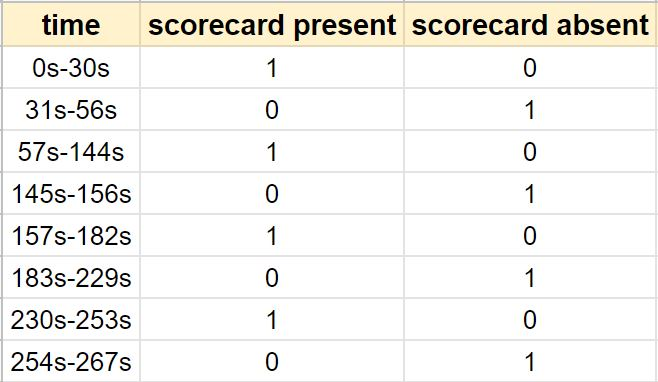
\includegraphics[width=0.8\textwidth,center]{out-preprocessing.jpg}
    \caption{Output of Preprocessing}
    \label{fig:out-preprocessing}
\end{figure}
\subsection{Visual Marker Detection}
The output of Visual Marker Detection module is shown in \ref{fig:out-Visual Marker Detection}. It shows frames with corresponding event tag and time.
\begin{figure}[h]
    \centering
   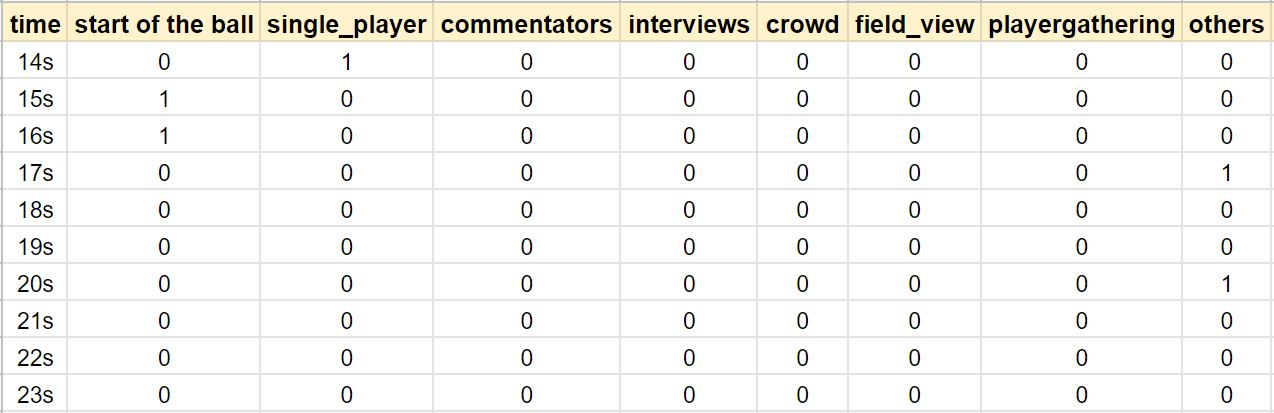
\includegraphics[width=1.0\textwidth,center]{out-frameannotation.jpg}
    \caption{Output of Visual Marker Detection}
    \label{fig:out-Visual Marker Detection}
\end{figure}

\subsection{Shot Boundary Detection and Segmentation}
The output of Shot Boundary Detection and Segmentation module is 'shown in \ref{fig:out-Ballboundary}. It shows every delivery in the input video.
\begin{figure}[h]
    \centering
   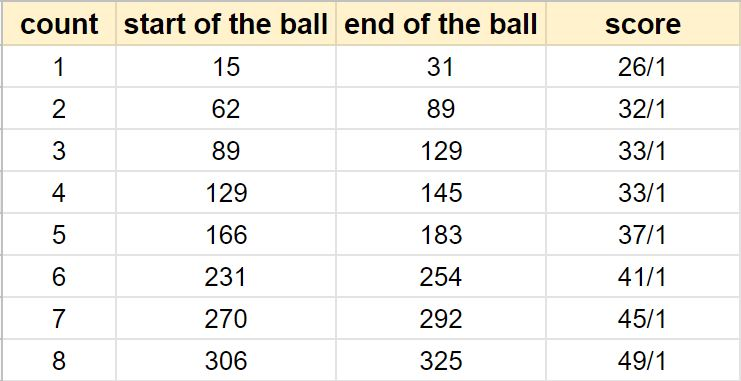
\includegraphics[width=0.9\textwidth,center]{out-ballboundary.jpg}
    \caption{Output of Shot Boundary Detection and Segmentation}
    \label{fig:out-Ballboundary}
\end{figure}
\subsection{Extraction of Highlights based on scorecard recognition}
The output of Extraction of Highlights based on scorecard recognition module is shown in \ref{fig:out-scorecard}. It shows delivery with highlights.
\begin{figure}[h]
    \centering
   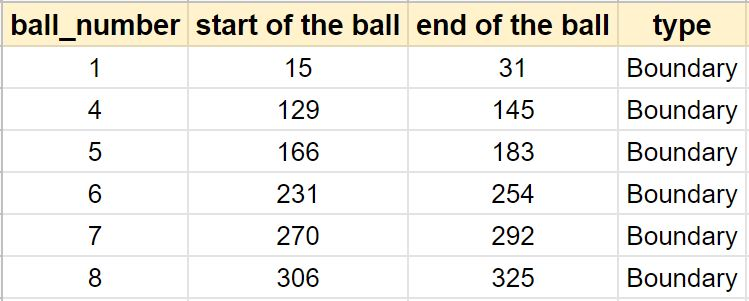
\includegraphics[width=0.9\textwidth,center]{out-scorecard.jpg}
    \caption{Output of Extraction of Highlights based on scorecard recognition}
    \label{fig:out-scorecard}
\end{figure}

\subsection{Extraction of Highlights based on excitement detection}
The output of Extraction of Highlights based on excitement detection module is shown in \ref{fig:out-excitement}. It shows delivery with highlights.
\begin{figure}[h]
    \centering
   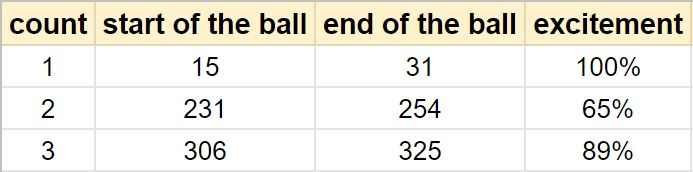
\includegraphics[width=0.9\textwidth,center]{out-excitement.jpg}
    \caption{Output of Extraction of Highlights based on excitement detection}
    \label{fig:out-excitement}
\end{figure}
\subsection{Aggregation of highlights}
The output of Aggregation of highlights module is shown in \ref{fig:out-Aggregation of highlights}. It shows delivery with highlights based on both scorecard and excitement
\begin{figure}[h]
    \centering
   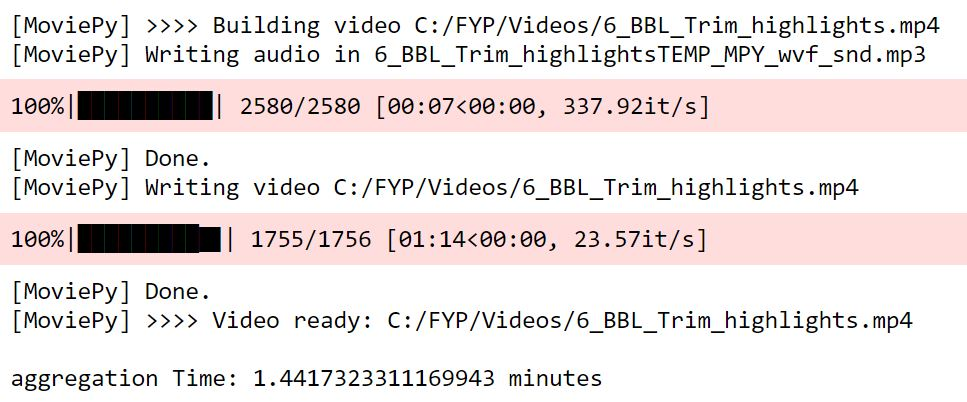
\includegraphics[width=1.0\textwidth,center]{out-aggregation.jpg}
    \caption{Output of Aggregation of highlights}
    \label{fig:out-Aggregation of highlights}
\end{figure}


\section{Results}
The system is developed using Python 3x. for programming and Keras package is used for building the CNNs. Moviepy tool is used for clipping and concatenating the highlights video. Various Big Bash League match videos are used to test the system. Day and night matches are selected to test whether the system can support matches with variations in the contrast. The networks are trained using more than 4000 images for event detection in each frame. The final highlights video which contains the excited and interesting segments are validated against the highlights video generated manually. Precision, recall, accuracy, error rates are used as evaluation metrics.
\section{Performance Evaluation}
The performance of the system is evaluated using two major categories objective evaluation, subjective evaluation.

Objective evaluation criterion relies on metrics such as precision, recall, accuracy, error rates, etc. to measure the performance of the system.Following are the some evaluation metrics:
\begin{itemize}
    \item \textbf {True Positive (TP):} It refers to the positive samples that are correctly labeled by the classifier.
    \item \textbf {True Negative (TN):} It refers to the negative samples that are correctly labeled by the classifier.
    \item \textbf {False Positive (FP):} It refers to the negative samples that are incorrectly labeled as positive by the classifier.
    \item \textbf {False Negative (FN):} It refers to the positive samples that are incorrectly labeled as negative by the classifier.
    \item \textbf {Precision Rate (PR):} It is a ratio of number of correctly labeled events (or frames), TP, to the total number of events detected.
      \[ Precision= \frac{TP}{TP+FP}\]
    \item \textbf {Recall Rate (RR):} It is a ratio of true detection rate with respect to the actual events (frames) in the video.
      \[ Recall= \frac{TP}{TP+FN}\]
    \item \textbf {Error Rate (ER): }It is a ratio of the miss labeled events (both false positives and false negatives) to the total number of events examined.
    \[ Error Rate= \frac{FP+FN}{TP+TN+FP+FN}\]
    \item \textbf {Accuracy Rate (AR):} It is a ratio of the correctly labeled events (both true positives and true negatives) to the total number of events.
      \[ Accuracy= \frac{TP+TN}{TP+TN+FP+FN}\]
\end{itemize}

\subsection{Preprocessing}
Table \ref{tab:Preprocessing - confusion matrix} contains result of the preprocessing module. In preprocessing module, live frames and Replay/Ads frames are detected and classified.
  %preprocessing
\begin{table}[ht]
\begin{center}
\begin{tabular}{@{}cc|ccc@{}}
\multicolumn{1}{c}{} &\multicolumn{1}{c}{} &\multicolumn{3}{c}{Predicted} \\ 
\multicolumn{1}{c}{} & 
\multicolumn{1}{c|}{} & 
\multicolumn{1}{c}{Live Frames} & 
\multicolumn{1}{c}{Replay/Ad Frames} & 
\multicolumn{1}{c}{Accuracy} \\ 
\cline{2-5}
\multirow{}{}{\rotatebox[origin=tr]{90}{Actual}}
& Live Frames  & 205 & 5 & 0  \\[1.5ex]
& Replay/Ad Frames  & 5  & 113 & 0\\ 
\cline{2-5}
\end{tabular}
\end{center}
\caption{Preprocessing - Confusion matrix}
\label{tab:Preprocessing - confusion matrix}
\end{table}
 
 \subsection{Visual Marker Detection}
Table \ref{tab:visual marker detection - confusion matrix} shows the result of visual marker detection where each live frame's event is detected. Here 1 represents start of the ball, 2 represents single player, 3 represents commentators, 4 represents interviews, 5 represents field view, 6 represents crowd, 7 represents player gathering, 8 represents other frames.
  %visual marker detection
\begin{table}[ht]
\begin{center}
    \begin{tabular}{@{}cc|ccccccccc@{}}
\multicolumn{1}{c}{} &\multicolumn{1}{c}{} &\multicolumn{9}{c}{Predicted} \\ 
\multicolumn{1}{c}{} & 
\multicolumn{1}{c|}{} & 
\multicolumn{1}{c}{1} & 
\multicolumn{1}{c}{2} & 
\multicolumn{1}{c}{3} &
\multicolumn{1}{c}{4} &
\multicolumn{1}{c}{5} &
\multicolumn{1}{c}{6} &
\multicolumn{1}{c}{7} &
\multicolumn{1}{c}{8} &
\multicolumn{1}{c}{Accuracy} \\ 
\cline{2-11}
\multirow{8}{}{\rotatebox[origin=c]{90}{Actual}}
& 1  & 45 & 0 & 0 & 9 & 0 & 0 & 0 & 6 & 83\\
& 2  &  0  & 24  & 3 & 0 & 3 & 0 & 0 & 0 & 91\\ 
& 3  & 0   & 6  & 18 & 0 & 3 & 3 & 0 & 0 & 88\\ 
& 4  & 9  & 0  & 0 & 18 & 0 & 3 & 0 & 0 & 88\\ 
& 5  & 0   & 0  & 6 & 0 & 21 & 3 & 0 & 0 & 87\\ 
& 6  & 0   & 3  & 0 & 0 & 6 & 21 & 0 & 0 & 90\\ 
& 7   & 0   & 6  & 18 & 0 & 3 & 3 & 0 & 0 & 88\\ 
& 8  & 9  & 0  & 0 & 0 & 0 & 0 & 0 & 7 & 0\\ 

\cline{2-11}
\end{tabular}

\end{center}
\caption{Visual Marker Detection - Confusion matrix}
\label{tab:visual marker detection - confusion matrix}
\end{table}

 \subsection{Shot boundary detection}
Table \ref{tab:shot boundary detection - confusion matrix} shows the result of shot boundary detection where shots are created using the event tag of the corresponding frames. Here each number represents its corresponding delivery's frames.
  %shot boundary detection
\begin{table}[ht]
\begin{center}
  \begin{tabular}{@{}cc|cccccccccc@{}}
\multicolumn{1}{c}{} &\multicolumn{1}{c}{} &\multicolumn{9}{c}{Predicted} \\ 
\multicolumn{1}{c}{} & 
\multicolumn{1}{c|}{} & 
\multicolumn{1}{c}{1} & 
\multicolumn{1}{c}{2} & 
\multicolumn{1}{c}{3} &
\multicolumn{1}{c}{4} &
\multicolumn{1}{c}{5} &
\multicolumn{1}{c}{6} &
\multicolumn{1}{c}{7} &
\multicolumn{1}{c}{8} &
\multicolumn{1}{c}{others} &
\multicolumn{1}{c}{Accuracy} \\ 
\cline{2-12}
\multirow{7}{}{\rotatebox[origin=c]{90}{Actual}}
& 1  & 15  & 0  & 0 & 0 & 0 & 0 & 0 & 4 &1 & 83\\
& 2  &  0  & 24 & 6 & 0 & 0 & 0 & 0 & 0 &1  & 91\\ 
& 3  & 0   & 0  & 33& 0 & 0 & 0 & 0 & 0 &0 & 88\\ 
& 4  & 6   & 0  & 1 & 14 & 0 & 0 & 0 & 0 &0 & 88\\ 
& 5  & 0   & 0  & 0 & 0 & 16 & 0 & 0 & 0 &0 & 87\\ 
& 6  & 0   & 0  & 0 & 0 & 0 & 20 & 0 & 0 &0 & 90\\ 
& 7  & 0   & 0  & 0 & 0 & 0 & 0 & 20 & 0 &0 & 88\\ 
& 8  &0    & 0  & 0 & 0 & 0 & 0 & 0 & 21 &0 & 0\\
& others   & 1  & 0 & 1 & 2 & 5 & 2 & 4 & 0 & 142 & 88\\ 
\cline{2-12}
\end{tabular}
\end{center}
\caption{Shot Boundary Detection - Confusion matrix}
\label{tab:shot boundary detection - confusion matrix}
\end{table}

\subsection{Extraction of Highlights Scorecard Recognition}
Table \ref{tab:scorecard recognition - Confusion matrix} shows the result of scorecard recognition where highlights shots are created using score present in the scorecard. Here each number represents its corresponding delivery's frames of the highlights.
%scorecard recognition
\begin{table}[ht]
\begin{center}
  \begin{tabular}
  {@{}cc|cccccccc@{}}
\multicolumn{1}{c}{} &\multicolumn{1}{c}{} &\multicolumn{7}{c}{Predicted} \\ 
\multicolumn{1}{c}{} & 
\multicolumn{1}{c|}{} & 
\multicolumn{1}{c}{1} & 
\multicolumn{1}{c}{4} &
\multicolumn{1}{c}{5} &
\multicolumn{1}{c}{6} &
\multicolumn{1}{c}{7} &
\multicolumn{1}{c}{8} &
\multicolumn{1}{c}{others} &
\multicolumn{1}{c}{Accuracy} \\ 
\cline{2-10}
\multirow{5}{}{\rotatebox[origin=c]{90}{Actual}}
& 1  & 15 & 0 & 0 & 0 & 0 & 4 &1 & 83\\
& 4  & 6   & 14 & 0 & 0 & 0 & 0 &1 & 88\\ 
& 5  & 0  & 0 & 16 & 0 & 0 & 0 &0 & 87\\ 
& 6  & 0   & 0 & 0 & 20 & 0 & 0 &0 & 90\\ 
& 7  & 0   & 0 & 0 & 0 & 20 & 0 &0 & 88\\ 
& 8  &0   & 0 & 0 & 0 & 0 & 21 &0 & 0\\
& others   & 1 & 2 & 5 & 2 & 4 & 0 & 206 & 88\\ 
\cline{2-10}

\end{tabular}
\end{center}
\caption{Scorecard Recognition - Confusion matrix}
\label{tab:scorecard recognition - Confusion matrix}
\end{table}
\subsection{Subjective Evaluation}
Subjective evaluation is based on user feedback score or rating. The subjective nature of this mechanism makes it difficult to define a benchmark as the quality parameters may vary among different users. 

We conducted a user study in order to determine the perceptual quality of the highlights generated by our approach. 10 highlights clips generated by our algorithm were shown to 20 different cricket fans in the age group of 20-60 years. The participants were asked to rate the clips from 0 to 5. The description of the rating is shown in table\ref{tab:userdescription}.
\begin{table}[ht]
\caption{Scale for user rating} % title of Table
\centering 
\begin{tabular}{lll} 
\hline
Score & Level  & Description \\ [0.5ex] % inserts table
\hline
5 & Perfect &  Good highlights  \\
4 & Fair &  Good highlights with few mistakes \\
3 & Acceptable &  Ok with both highlights and boring segments\\
2 & Bad &   Highlights with some unwanted segments \\
1 & Poor &  Highlights with many unwanted segments \\
0 & Very poor & Most of the highlight segments are boring\\[1ex]
\hline 
\end{tabular}
\label{tab:userdescription}
\end{table}

\section{Discussion}
Precision and recall \ref{graph:prerecall}.\\
\newline
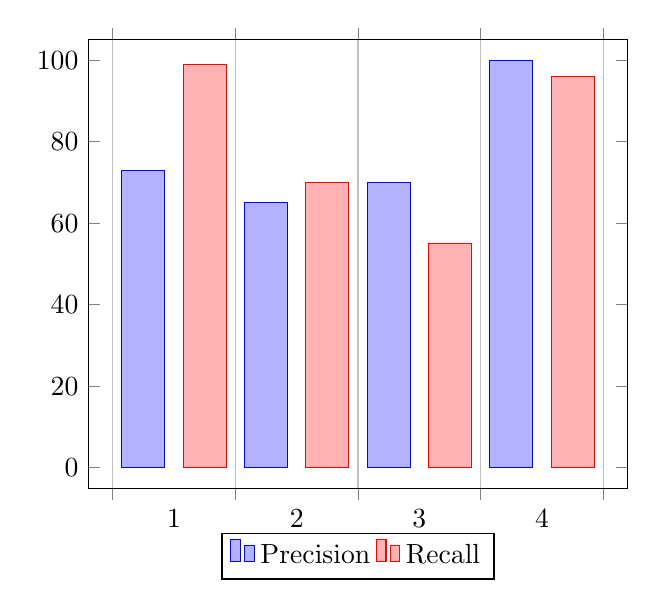
\begin{tikzpicture}
\begin{axis}[
	x tick label style={
		/pgf/number format/1000 sep=},
	ymin=0, ymax=100,
	ylabel,
	enlargelimits=0.05,
	legend style={at={(0.5,-0.1)},
	anchor=north,legend columns=-1},
	ybar interval=0.7,
]
\addplot coordinates {(1,73) (2,65) (3,70) (4,100) (5,86)};   
\addplot coordinates {(1,99) (2,70) (3,55) (4,96) (5,81)};   
\legend{Precision, Recall}
\end{axis}
\label{graph:prerecall}
\end{tikzpicture}

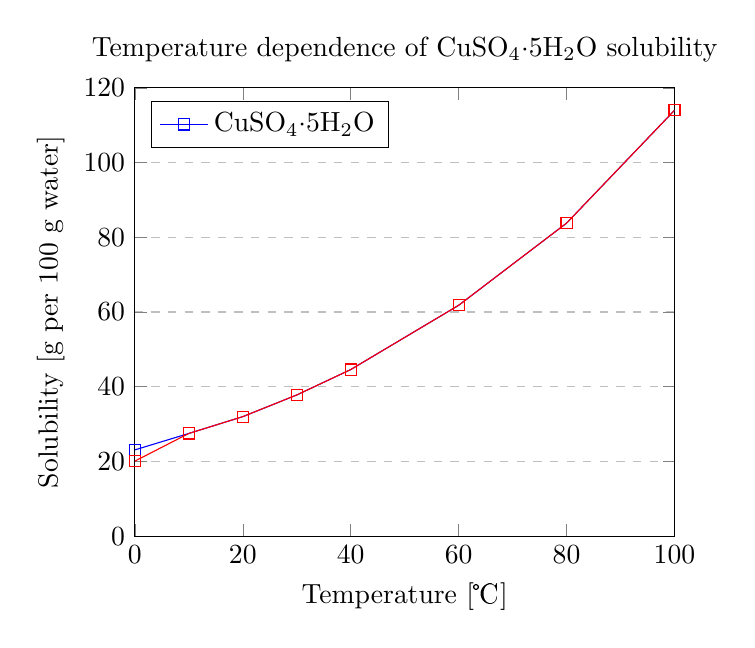
\begin{tikzpicture}
\begin{axis}[
    title={Temperature dependence of CuSO$_4\cdot$5H$_2$O solubility},
    xlabel={Temperature [\textcelsius]},
    ylabel={Solubility [g per 100 g water]},
    xmin=0, xmax=100,
    ymin=0, ymax=120,
    xtick={0,20,40,60,80,100},
    ytick={0,20,40,60,80,100,120},
    legend pos=north west,
    ymajorgrids=true,
    grid style=dashed,
]
 
\addplot[
    color=blue,
    mark=square,
    ]
    coordinates {
    (0,23.1)(10,27.5)(20,32)(30,37.8)(40,44.6)(60,61.8)(80,83.8)(100,114)
    };
    \legend{CuSO$_4\cdot$5H$_2$O}
 
 \addplot[
    color=red,
    mark=square,
    ]
    coordinates {
    (0,20.1)(10,27.5)(20,32)(30,37.8)(40,44.6)(60,61.8)(80,83.8)(100,114)
    };
    \legend{CuSO$_4\cdot$5H$_2$O}
 
\end{axis}
\end{tikzpicture}